
\documentclass{article}
\usepackage{polski}
\usepackage[utf8]{inputenc}
\usepackage{enumerate}
\usepackage{blindtext}
\usepackage{graphicx}
\usepackage{geometry}
\usepackage{listings}
\usepackage{float}
\usepackage[table]{xcolor}
\setlength{\parskip}{0pt} 
\newgeometry{lmargin = 3cm, rmargin=2.5cm}
\renewcommand{\labelenumi}{\arabic{enumi}.}
\renewcommand{\labelenumii}{\arabic{enumi}.\arabic{enumii}.}


\begin{document}
\begin{titlepage}
	\centering
	
\includegraphics[width=0.15\textwidth]{agh}\par\vspace{1cm}	
	{\scshape\large AKADEMIA GÓRNICZO-HUTNICZA \\IM. STANISŁAWA STASZICA W KRAKOWIE \par}
	\vspace{0.5cm}
	{\scshape\large Wydział elektrotechniki automatyki	informatyki i inżynierii biomedycznej \par}
	\vspace{0.5cm}
	{\scshape\Large Informatyka \par}
	\vspace{1cm}
	{\huge\bfseries Wykorzystanie SAT Solverów w tworzeniu harmonogramów\par}
	\vspace{2cm}
	{\large Izabela Kiełbasa \\ Natalia Janecka\par}
	\vfill
	\vfill
	{\large \today\par}
\end{titlepage}
%%\tableofcontents
\clearpage
\section{Użycie SAT Solvera w projekcie}
\par
Do rozwiązywania problemów SAT w projekcie została wykorzystana biblioteka dla Javy: \textbf{Sat4j}. Umożliwia ona rozwiązywanie problemów satysfakcji zdań logicznych oraz optymalizacji. Pozwala na rozwiązanie problemów SAT, MAXSAT, Pseudo-Boolean oraz Minimally Unsatisfable Subset (MUS). \\
Biblioteka ta jest przyjazna dla użytkownika i zaprojektowana elastycznie używając wzorców projektowych takich jak dekorator i strategia. Jej zaletą jest również to, że jest open source. \\ \\
SAT przyjmuje zdanie logoczne w formie \textbf{CNF} – koniunkcyjna postać normalna. Formuła zapisana w koniunkcji klauzul np.: $$ (x1 \vee x2 \vee x3) \wedge (x4 \vee x2) $$
Każda formuła CNF składa się ze \textbf{zmiennych}, które mogą przyjmować tylko wartości \textbf{\textit{prawda}} lub \textbf{\textit{fałsz}} (dla powyższego przykładu jest ich 4) oraz \textbf{klauzul} na zmiennych np.: $$ C1\wedge C2\wedge ...\wedge Cn $$(dla powyższego przykładu mamy 2 klauzule). \\ \\
SAT znajduje rozwiązanie dla podanego zdania tak aby cała formuła była prawdziwa (wszystkie klauzule muszą być prawdziwe). Jeśli rozwiązanie nie istnieje to SAT zwraca odpowiednią informację. \\
MAXSAT znajduje jak najwięszką ilość zmiennych tak aby zdanie było prawdziwe. Natomiast MUS znajduje jak najmiejszą ilość zmiennych dla której zdanie jest niespełnione. \\ \\
\par
Bibioteka sat4j przyjmuje jako wejście plik o rozszerzeniu \textbf{.cnf}. Plik ten składa się z 2 części:\textit{ preambuły} oraz \textit{klauzul}. 
\begin{enumerate}
\item \underline{Preambuła} zawiera informacje na temat przykładu. Każda linia zaczyna się od litery która ją charakteryzuje. 
\begin{itemize}
	\item Linia komentarza zaczyna się od litery “c” a po niej nastepuje spacja i komentarz
	\item 
 Problem line – jedna linia dla pliku, definiuje zawartość pliku. Dla pliku CNF wygląda ona natępująco:
\begin{lstlisting}
p cnf iloscZmiennych iloscKlauzul 
\end{lstlisting} 
\end{itemize} 
\item
Druga część pliku to \underline{część klauzul} – pojawia się ona bezpośrednio po linii problemu. Zmienne są ponumerowane od 1 do n (gdzie n to ilość zmiennych). Każda klauzula jest reprezentowana jako sekwencja liczb, oddzielonych od siebie spacją, tabem lub znakiem nowej linii. Zmienna prawdziwa jest zapisywana jako $i$,  a zmienna fałszywa jako $\neg i$. Każda klauzula jest zakończona wartością 0. 
Dla powyzszego przykładu plik .cnf ma postać
\begin{lstlisting}
	p cnf 4 2
	1 2 3 0
	4 2 0
\end{lstlisting}

Jako rozwiązanie SATa będzie tu przedstawiona linia
\begin{lstlisting}
1 2 3 4 0
\end{lstlisting}

co oznacza, że aby dana formuła była prawdziwa wszystkie jej zmienne muszą być prawdziwe.  Jeśli przed którąś ze zmiennych byłby znak "$\neg$" to zmienna ta powinna być fałszywa aby formuła była spełniona. 
\end{enumerate}


\section{Słownik pojęć}
\par
\begin{itemize}
	\item Instruktor - osoba pracująca, która prowadzi jazdy, ma określone godziny pracy(patrz niżej), jednocześnie może prowadzić zajęcia tylko z jednym kursantem
	\item Kursant - osoba uczestnicząca w zajęciach, może na każdą jazdę wybrać jednego instruktora z listy. Ma określone preferowane godziny zajęć(patrz niżej). Ostateczna godzina zajęć zostanie wybrana z listy preferowanych przez kursanta jeśli wybrany przez niego instruktor jest wtedy dostępny. Kursant może mieć tylko jedne zajęcia dziennie.  
	\item Godziny pracy instruktora - pary: data i godzina rozpoczęcia oraz zakończenia pracy. Pierwszy termin zawsze musi być wcześniejszy niż drugi. Może być kilka takich par dla jednego dnia - oznacza to, że instruktor pracuje z przerwami w godzinach, które nie zawierają sie pomiędzy godzinami w parach.
	\item Preferowane godziny zajęć - pary: data i godzina rozpoczęcia i zakończenia jazdy. W tym czasie kursant może odbywać jazdy. Może być kilka wylistowanych. Dla konkretnego dnia wybrana zostanie tylko jedna para. Zajęcia nie mogą trwać dłużej niż jeden dzień. Czas rozpoczęcia nie może być ustawiony na pózniejszy niż czas zakończenia.

\end{itemize}
\section{Tworzenie harmonogramu jazd}
\par
W aplikacji mamy wybór między dwoma sposobami wprowadzenia danych: manualne dodawanie instruktorów, godzin ich pracy oraz studentów i ich preferowanych godzin zajęć; oraz poprzez wczytanie plików .csv z gotowymi danymi.
Każdemu z tych sposobów odpowiada osobna karta. \\
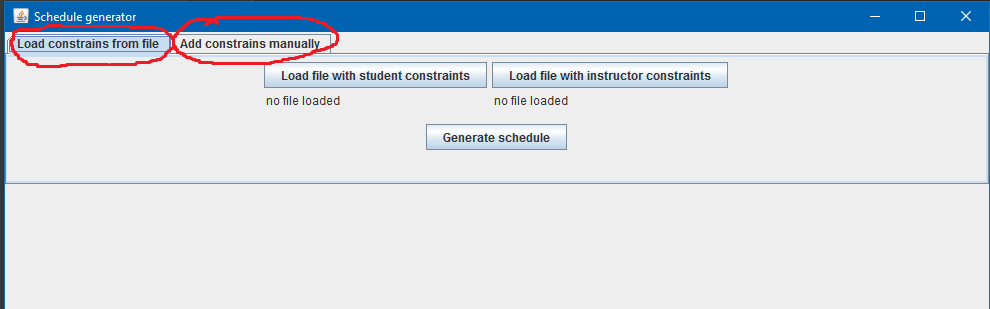
\includegraphics[width=0.7\textwidth]{screen-karty.png} \\ \\
\newpage
Domyślnie najpierw otwiera się karta z opcją wczytania danych z pliku. Po naciśnięciu odpowiednich przycisków otworzą się okienka do wyszukiwania plików .csv z planem odpowiednio dla studentów i instruktorów. Po wybraniu pliku pod przyciskiem pojawi się jego nazwa. \\ 
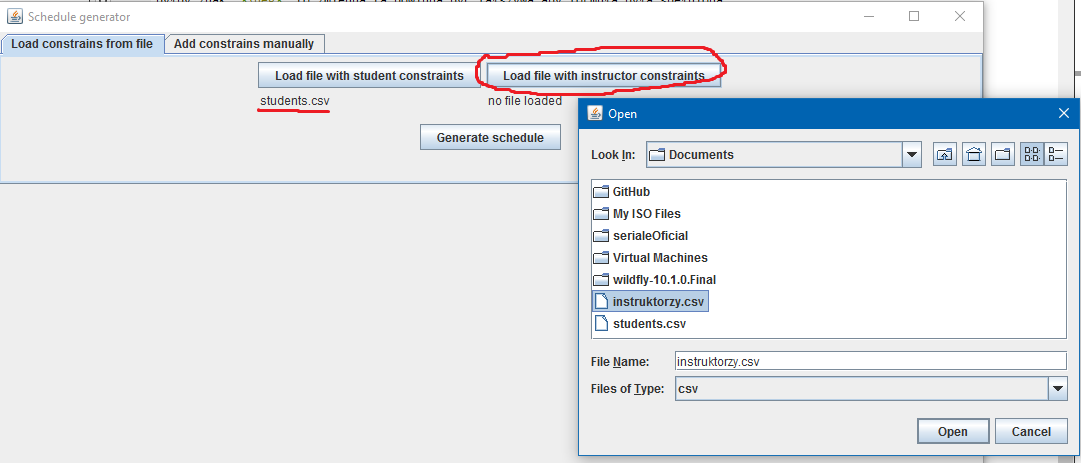
\includegraphics[width=0.7\textwidth]{screen-openFile.png} \\ \\ 
Po wybraniu obu plików z danymi naciskamy przycisk \textit{Generate schedule} co spowoduje otwarcie nowego okienka z wygenerowanym harmonogramem opartym na naszych danych.\\
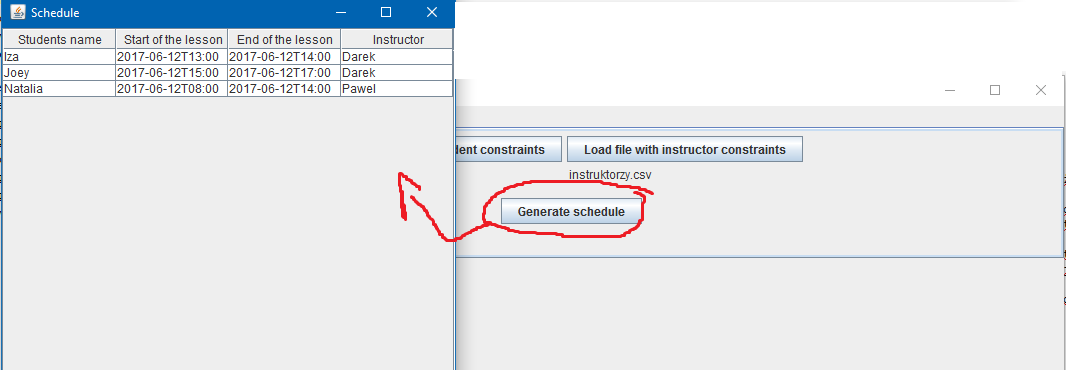
\includegraphics[width=0.5\textwidth]{screen-generate1.png} \\
\\
Plik formatu csv stworzony na przykład w Exelu ma taką postać:\\ 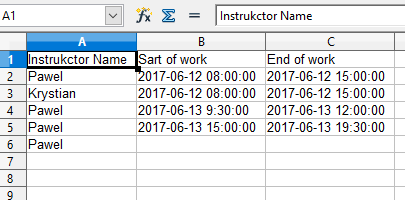
\includegraphics[width=0.5\textwidth]{dane-inst.png}

\newpage
\par
Jeśli chcemy dodać dane ręcznie wybieramy drugą zakładkę. Pojawią sie nam kolejne dwie zakładki. W pierwszej możemy dodać instruktorów i wybrać dla nich godziny pracy.\\
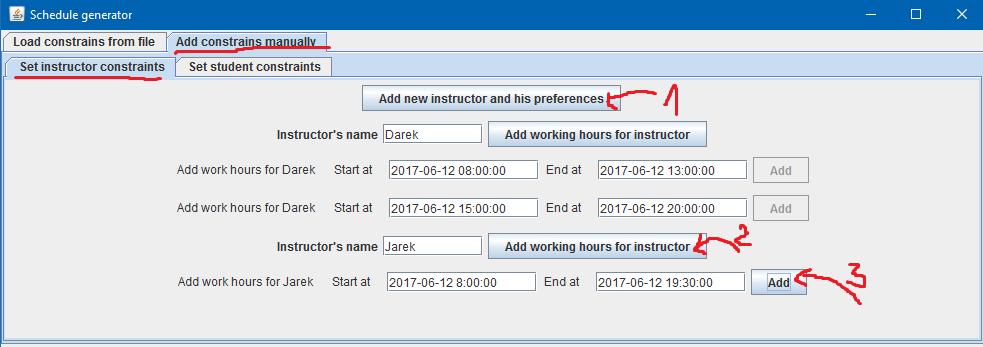
\includegraphics[width=0.7\textwidth]{screen-inst.png} \\ \\ 
Przyciskiem na samej górze(1) dodajemy nowego instruktora, podajemy jego imię, a następnie dodajemy godziny pracy przyciskiem(2). Uzupełniamy datę i godzinę początku i końca w formacie yyyy-MM-dd HH:mm:ss. Jeśli instruktor ma przerwę w pracy możemy dodać kilka zakresów czasu, w którym pracuje. Aby dodać ograniczenia czasowe klikamy przycisk (3). \\ \\ \\



W drugiej zakładce można dodać kursantów. Za pomoca przycisku (1) dodajemy nowego kursanta i nadajemy mu imię. Następnie wybieramy (2) i dodajemy preferowane godziny zajęć oraz instruktora z listy(4). Po wpisaniu danych zatwierdzamy je przyciskiem(3). Jeśli chcemy dodać kolejny preferowany przedział czasowy ponownie klikamy(2/5). \\ 
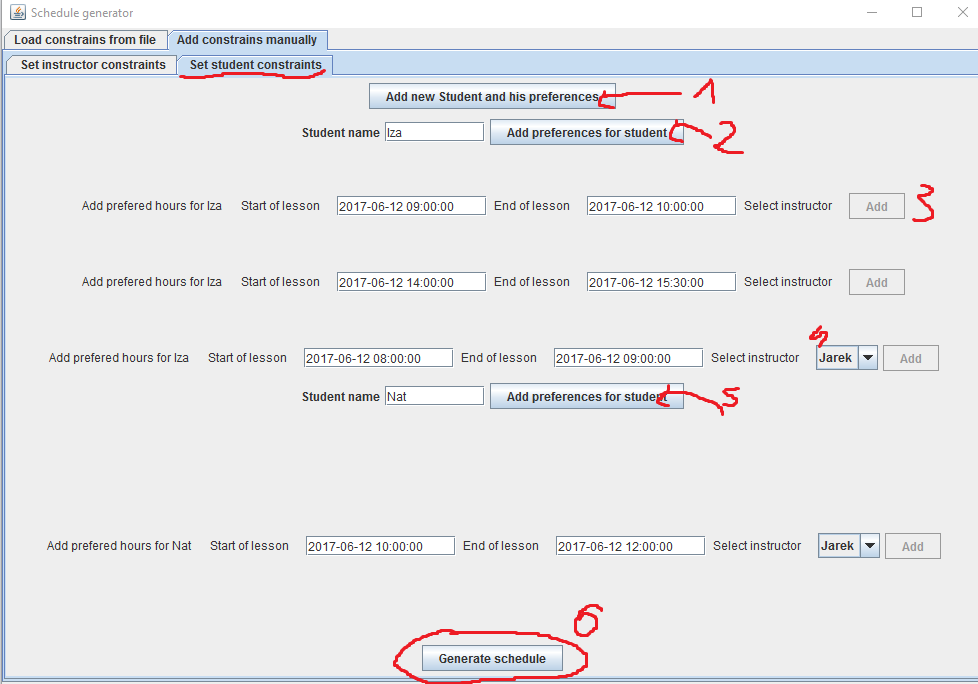
\includegraphics[width=0.7\textwidth]{screen-stud.png} \\ \\ 

Kiedy dodaliśmy już wszystkie preferencje klikamy przycisk $Generate$(6). W nowym okienku pokaże nam się wygenerowany przez SAT grafik, który spełnia wszystkie ograniczenia. \\ Wynikowa tabelka jest posortowana według instruktorów, a następnie godzin rozpoczęcia jazdy. \\ \\
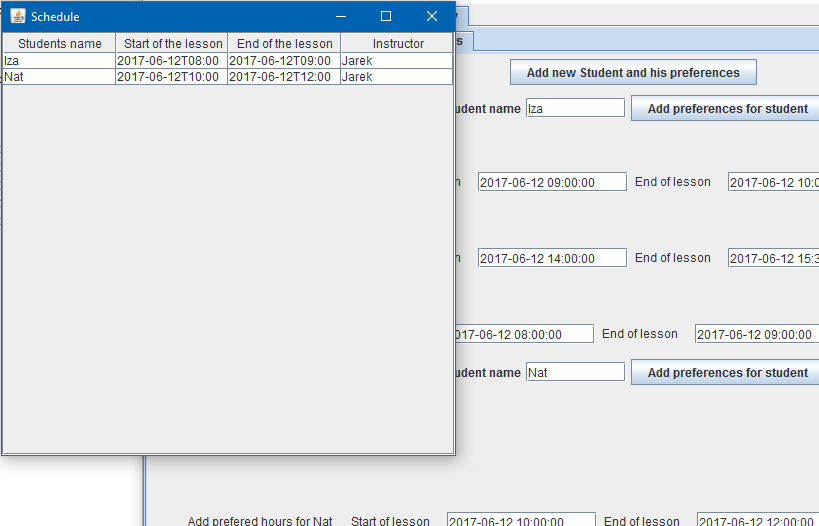
\includegraphics[width=0.5\textwidth]{screen-schedule.png} \\
Jeśli nie da się spełnić wszystkich ograniczeń pojawi się okienko: 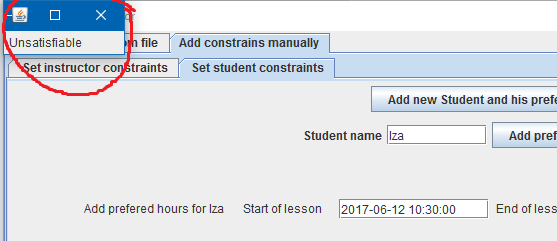
\includegraphics[width=0.5\textwidth]{screen-unsatisfiable.png}
\end{document}